\chapter{Evaluation}
\label{chap:Evaluation}

We assert that by enhancing the abstraction level of model and property specifications, cascading verification also enhances the effectiveness of probabilistic model checking. To validate this assertion, we will demonstrate that, as an implementation of cascading verification for the UAV domain, the prototype presented in this thesis benefits mission developers by simplifying the verification of UAV mission plans, and by augmenting PRISM's verification capabilities. Ultimately, we aim to show that our prototype benefits mission developers by improving the correctness of UAV mission specifications. We will also evaluate the portability of cascading verification, i.e., the usability of our method in the context of different application domains.

The remainder of this chapter is structured as follows. Section~\ref{sec:Evaluation_Methods_and_Metrics} describes the methodologies and metrics that underpin the evaluation of our method and prototype. Limitations and threats to the validity of the evaluation are presented in Section~\ref{sec:Threats_to_Validity}. This chapter is summarized in Section~\ref{sec:Evaluation_Summary}.

\section{Evaluation Methods and Metrics}
\label{sec:Evaluation_Methods_and_Metrics}

This evaluation focuses on a single project, and assesses the effects of change prior to large-scale implementation and deployment. Case studies therefore constitute an appropriate evaluation method~\cite{Kitchenham_1995}. Importantly, case studies 1) avoid scalability issues associated with the evaluation of software-engineering tools and methods, and 2) support high-level assessments, which are desirable for wide-ranging process changes. The evaluation was not affected by ancillary budgetary, scheduling and staffing issues.

\subsection{Abstraction}

Because it was unfeasible to involve practitioners in the evaluation of our prototype's utility, we opted instead for a metrics-based analysis of~58 mission plans. These plans were based on real-world mission scenarios developed independently by DARPA and DRDC~\cite{DARPA,Youngson_2004}. We evaluated our approach by comparing the LOC and numbers of lexical tokens required to specify missions in YAML against the LOC and tokens in the combined DTMC and PCTL code synthesized by the CVC\@. On average, our prototype synthesizes PRISM code that is 3.127 and 4.490 times greater than the size of YAML input with regard to LOC and tokens, respectively. (The standard deviations were 52.4\% and 95.4\%, respectively.) These results provide preliminary evidence of non-trivial reduction in the effort required to produce mission models and properties.

Table~\ref{tab:mission_metrics} lists metric values for a subset of the~58 mission plans. This subset represents the full range of observed PRISM-to-YAML ratios. (Appendix~\ref{chap:Mission_Verification_Artifacts} contains verification artifacts---including mission specifications encoded in YAML, synthesized DTMC and PCTL artifacts, and PRISM results---for the mission plans presented in Table~\ref{tab:mission_metrics}.)

\begin{table}[ht]
	\arrayrulecolor{Gray}
	\renewcommand*\arraystretch{1.3}
	\begin{tabularx}{\textwidth}{
			>{\centering\hsize=0.08\hsize}X|
			>{\centering\hsize=0.14\hsize}X
			>{\centering\hsize=0.14\hsize}X|
			>{\centering\hsize=0.14\hsize}X
			>{\centering\hsize=0.14\hsize}X|
			>{\centering\hsize=0.18\hsize}X
			>{\centering\hsize=0.18\hsize}X
		}
		& \multicolumn{2}{ c | }{YAML} &
			\multicolumn{2}{ c | }{PRISM} &
			\multicolumn{2}{ c }{PRISM-to-YAML ratio}\tabularnewline
		id & LOC & tokens & LOC & tokens & LOC & tokens\tabularnewline
		\hline
		1a & 9 & 31 & 22 & 104 & 244.4\% & 335.5\%\tabularnewline
		1d & 12 & 45 & 32 & 169 & 266.7\% & 375.6\%\tabularnewline
		1g & 15 & 59 & 36 & 218 & 240.0\% & 369.5\%\tabularnewline
		2a & 18 & 70 & 45 & 255 & 250.0\% & 364.3\%\tabularnewline
		2b & 18 & 72 & 52 & 277 & 288.9\% & 384.7\%\tabularnewline
		2e & 23 & 97 & 57 & 331 & 247.8\% & 341.2\%\tabularnewline
		2g & 25 & 105 & 77 & 457 & 308.0\% & 435.2\%\tabularnewline
		2j & 23 & 98 & 76 & 443 & 330.4\% & 452.0\%\tabularnewline
		2m & 26 & 112 & 91 & 558 & 350.0\% & 498.2\%\tabularnewline
		2p & 26 & 114 & 91 & 562 & 350.0\% & 493.0\%\tabularnewline
		2r & 25 & 109 & 84 & 468 & 336.0\% & 429.4\%\tabularnewline
		2u & 28 & 123 & 94 & 533 & 335.7\% & 433.3\%\tabularnewline
		2v & 28 & 123 & 99 & 583 & 353.6\% & 474.0\%\tabularnewline
		2w & 31 & 137 & 111 & 666 & 358.1\% & 486.1\%\tabularnewline
		2x & 31 & 137 & 111 & 666 & 358.1\% & 486.1\%\tabularnewline
		3a & 12 & 42 & 32 & 158 & 266.7\% & 376.2\%\tabularnewline
		3e & 15 & 56 & 45 & 252 & 300.0\% & 450.0\%\tabularnewline
		3h & 16 & 61 & 42 & 227 & 262.5\% & 372.1\%\tabularnewline
		3k & 18 & 70 & 60 & 357 & 333.3\% & 510.0\%\tabularnewline
		3o & 18 & 72 & 60 & 373 & 333.3\% & 518.1\%\tabularnewline
		4a & 21 & 94 & 39 & 267 & 185.7\% & 284.0\%\tabularnewline
		4b & 21 & 94 & 73 & 513 & 347.6\% & 545.7\%\tabularnewline
		4d & 25 & 110 & 100 & 707 & 400.0\% & 642.7\%\tabularnewline
		4f & 28 & 124 & 111 & 788 & 396.4\% & 635.5\%\tabularnewline
		5a & 23 & 92 & 58 & 329 & 252.2\% & 357.6\%\tabularnewline
		5b & 23 & 92 & 104 & 744 & 452.2\% & 808.7\%\tabularnewline
	\end{tabularx}
	\caption[Mission plan metric values]{Metric values for representative mission plans.}
	\label{tab:mission_metrics}
\end{table}

We observe that tactical missions (4b, 4d and~4f in Table~\ref{tab:mission_metrics}) and traffic surveillance missions (5a and~5b) generate more LOC and tokens than \emph{standalone mission plans}, which are mission plans underpinned exclusively by CEMO and thereby not associated with the more specialized subdomains encoded in Tactical- and Traffic-CEMO\@. Specifically, tactical mission plans generate PRISM code that is on average 3.933 and 5.992 times greater than the size of YAML input with regard to LOC and tokens, respectively. (The standard deviations were 24.0\% and 59.2\%, respectively.) Mission~5b generates PRISM code that is 4.522 and 8.087 times greater than the size of YAML input with regard to LOC and tokens, respectively. Because the effort required to synthesize PRISM code is proportional to the effort required to synthesize the LOC and tokens that constitute the code, tactical and traffic surveillance mission plans result in added value for mission developers. This observation suggests that, with respect to tactical missions, the utility of our prototype is proportional to the threat level associated with any given mission plan. More broadly, increased LOC and token output suggests that the utility of cascading verification may be proportional to the amount of automated reasoning required to synthesize pertinent artifacts, a conclusion that justifies our motivation to augment model checking with formalized domain knowledge.

\subsection{Effectiveness}

Because it cannot account for the intricate syntax of the PRISM language, a LOC- and token-based analysis offers limited insight into the inherent complexity of model and property specifications. We investigate complexity further by considering \emph{behavioral modeling errors} specific to the PRISM language that can be eliminated with the automated synthesis of PRISM artifacts (at least for the segment of the mission space that we have explored thus far). These errors are significant, perhaps more so than the errors uncovered during the model checking process, because they can mislead mission developers by causing PRISM to verify erroneous mission plans.

In the context of the PRISM language and the PRISM models created for this project:

\begin{itemize}

\item\emph{Inconsistent variable errors} occur when PRISM variables are inconsistent in value with corresponding variables in mission specifications; for example, the duration of an action specified in YAML should be consistent in value with the local variable of the PRISM module corresponding to that action.\footnote{Action duration in the context of behavioral modeling was described in Section~\ref{sec:Behavioral_Modeling}.}

\item\emph{Command action errors} occur when command actions, which affect module synchronization, are incorrect across two or more modules.

\item\emph{Command probability errors} occur when commands are annotated with probabilities that fail to accurately reflect the system being modeled; for example, the probabilities encapsulated in an asset survivability module should accurately reflect the vulnerability of the asset corresponding to that module.\footnote{Asset survivability was described in Section~\ref{sec:Modeling_Tactical_Missions}.}

\item\emph{Command update errors} occur when command updates, which affect module behavior, are incomplete or incorrect. For example, an incomplete update could fail to couple the modules corresponding to an asset and the action assigned to that asset; an incorrect update could couple modules corresponding to an asset and an action assigned to a different asset.

\end{itemize}

We also consider mission specification errors that are beyond the scope of PRISM's verification capabilities. These \emph{domain-specific errors} are detected by either Pellet or the SWI-Prolog compiler during the synthesis process. We have identified 28 domain-specific errors, across six error classes, that impact the correctness of UAV missions. In the context of the OWL language and CEMO:

{
\parindent=0em

\newcommand{\myindent}[1]{\hangindent=2em\emph{#1}}

\myindent{Disjoint class errors} occur when individuals are declared in system specifications to be instances of incompatible classes; for example, a hover action can also be a kinetic action, but not a sensor action. This error type affects mission correctness by ambiguating mission constructs for humans and, potentially, computers. Construct ambiguity could, for example, cause humans to confuse action subtypes and thereby develop mission plans comprising one or more sensor actions and zero kinetic actions; without appropriate verification, automated processes could subsequently attempt to deploy erroneous missions that violate asset constraints related to the execution of kinetic actions (as described in Section~\ref{sec:Semantic_Modeling}). The OWL statements in Listing~\ref{lst:disjoint_classes} formally define disjoint classes that can cause domain-specific errors.

\begin{lstlisting}[caption={Disjoint class statements specified in OWL},label=lst:disjoint_classes]
Action DisjointWith Asset
ARDrone DisjointWith Hummingbird
HoverAction DisjointWith TraversePathSegmentAction
HoverAction DisjointWith LidarAction
HoverAction DisjointWith PhotoSurveillanceAction
TraversePathSegmentAction DisjointWith LidarAction
TraversePathSegmentAction DisjointWith PhotoSurveillanceAction
LidarAction DisjointWith PhotoSurveillanceAction
\end{lstlisting}

\myindent{Existential restriction errors} occur when individuals fail to participate in mandatory relationships, as specified by the OWL keyword \texttt{some}; for example, every asset must execute at least one kinetic action. The OWL statements in Listing~\ref{lst:existential_restrictions_in_OWL} formally define existential restrictions that can cause domain-specific errors. Because of OWA, which was described in Section~\ref{sec:OWL_SWRL_and_Prolog}, OWL-based reasoning cannot conclude the absence of a mandatory relationship from the absence of knowledge about that relationship. Consequently, existential restriction errors are detected exclusively by the SWI-Prolog compiler. The Prolog rules in Listing~\ref{lst:existential_restrictions_in_Prolog} encompass atoms that correspond to the existential restrictions in Listing~\ref{lst:existential_restrictions_in_OWL}.

\begin{figure}[ht]
\begin{lstlisting}[caption={Existential restriction statements specified in OWL},label=lst:existential_restrictions_in_OWL]
Asset hasAction some KineticAction
Asset hasEnduranceInSeconds some int
HoverAction hasWaypoint some Waypoint
KineticAction hasDurationInSeconds some int
LidarAction hasIntervalInSeconds some int
LidarAction isConcurrentWith some HoverAction
Mission hasAsset some Asset
PhotoSurveillanceAction hasDurationInSeconds some int
TraversePathSegmentAction hasEndpoint some Waypoint
TraversePathSegmentAction hasStartPoint some Waypoint
\end{lstlisting}
\end{figure}

\begin{figure}[ht]
\begin{lstlisting}[caption={Existential restrictions encompassed in Prolog rules},label=lst:existential_restrictions_in_Prolog]
invalid_asset(A) :-
    zero_action_asset(A);
    not(has_endurance_in_seconds(A, _)).

invalid_hover_action(H) :-
    invalid_kinetic_action(H);
    not(has_waypoint(H, _)).

invalid_kinetic_action(K) :-
    not(has_duration_in_seconds(K, _)).

invalid_lidar_action(L) :-
    not(has_interval_in_seconds(L, _));
    not(is_concurrent_with(L, _)).

invalid_mission(M) :-
    not(has_asset(M, _)).

invalid_photo_surveillance_action(P) :-
    not(has_duration_in_seconds(P, _)).

invalid_traverse_path_segmentAction(T) :-
    invalid_kinetic_action(T);
    not(has_endpoint(T, _));
    not(has_start_point(T, _)).
\end{lstlisting}
\end{figure}

\myindent{Data property value errors} occur when data property values declared in system specifications fall outside the ranges of corresponding data properties encoded in CEMO; for example, the endurance of a Hummingbird is 1200 time-steps. The OWL statements in Listing~\ref{lst:data_property_values} formally define data properties that can cause domain-specific errors.

\begin{figure}[ht]
\begin{lstlisting}[caption={Data property statements specified in OWL},label=lst:data_property_values]
ARDrone hasEnduranceInSeconds some int[<= 70]
Hummingbird hasEnduranceInSeconds some int[<= 120]
\end{lstlisting}
\end{figure}

\myindent{Data property domain and range errors} occur when data property domain and range types declared in system specifications are inconsistent with the domain and range types of the corresponding data properties encoded in CEMO; for example, CEMO specifies that every \texttt{Hummingbird} individual must be associated with a datatype property \texttt{hasCostValue} of type \texttt{int}. The OWL code in Listing~\ref{lst:data_properties} formally defines data properties that can cause domain-specific errors.

\begin{figure}[ht]
\begin{lstlisting}[caption={Data properties specified in OWL},label=lst:data_properties]
DataProperty: hasDurationInSeconds
  Characteristics: Functional
  Domain: Action
  Range: int

DataProperty: hasEnduranceInSeconds
  Characteristics: Functional
  Domain: Asset
  Range: int

DataProperty: hasIntervalInSeconds
  Characteristics: Functional
  Domain: LidarAction
  Range: int
\end{lstlisting}
\end{figure}

\myindent{Object property domain and range errors} occur when object property domain and range types declared in system specifications are inconsistent with the domain and range types of the corresponding object properties encoded in CEMO; for example, CEMO specifies that the object property \texttt{hasAction} associates every member of class \texttt{Asset} (the domain of \texttt{hasAction}) with a member of class \texttt{KineticAction} (the range). The OWL code in Listing~\ref{lst:object_properties} formally defines object properties that can cause domain-specific errors.

\begin{figure}[ht]
\begin{lstlisting}[caption={Object properties specified in OWL},label=lst:object_properties]
ObjectProperty: hasAction
  Characteristics: Asymmetric, Irreflexive, InverseFunctional
  Domain: Asset
  Range: Action
  InverseOf: isActionOf

ObjectProperty: hasAsset
  Characteristics: Asymmetric, Irreflexive, InverseFunctional
  Domain: Mission
  Range: Asset

ObjectProperty: hasPrecondition
  Characteristics: Transitive
  Domain: Action
  Range: Action
  InverseOf: isPreconditionTo

ObjectProperty: isConcurrentWith
  Characteristics: Asymmetric, Irreflexive
  Domain: LidarAction
  Range: HoverAction
\end{lstlisting}
\end{figure}

\myindent{Threatened asset errors} occur when mission plans comprise a threatened asset that is not also a valid asset.\footnote{Threatened and valid assets were described in Section~\ref{sec:Modeling_Tactical_Missions}.} With the exception of this UAV-related error class, domain-specific errors are caused by inconsistencies between a mission specification and the underlying domain model. Given adequate documentation of the YAML DSL, these inconsistencies could, in theory, be eliminated by mission developers during the design and implementation of mission plans (in practice, software bugs elude extinction). But threatened and valid assets can only be discovered with geodetic calculations and subsequent formal reasoning, as described in Section~\ref{sec:From_Specification_to_Verification} and Section~\ref{sec:Modeling_Tactical_Missions}, respectively. The OWL code in Listing~\ref{lst:OWL_class_ThreatenedAsset} formally defines class \texttt{ThreatenedAsset}.

}

\begin{figure}[ht]
\begin{lstlisting}[caption={OWL code for class \texttt{ThreatenedAsset}},label=lst:OWL_class_ThreatenedAsset]
Class: ThreatenedAsset
  EquivalentTo: Asset
    and (hasAction some DirectThreatAreaHoverAction)
  DisjointWith: DirectThreatAreaTPSA
\end{lstlisting}
\end{figure}

Mission correctness can clearly be compromised by domain-specific and behavioral modeling errors, which occur during the design/implementation and verification phases, respectively, of the mission development process. Our prototype augments PRISM's effectiveness by preventing both of these error types.

\subsection{Probabilistic Verification}

Finally, we consider PRISM's ability to meaningfully verify UAV mission plans (or rather, we consider the utility of the DTMC and PCTL artifacts synthesized by our prototype). For this part of the evaluation, eighteen of the~58 mission plans described above were seeded with errors, including deadlock and non-reachable states, that violated desirable behavioral properties. One mission plan failed (i.e., contained errors that resulted in a 0.0 probability of success) because of an unacceptably low RAF value.\footnote{The RAF value was described in Section~\ref{sec:Verification_with_Semantic_Reasoning}.}

Nine mission plans failed because kinetic or sensor action workflow durations exceeded the endurances of the assets to which those workflows were assigned. Figure~\ref{fig:mission_3g} illustrates this type of error with Mission~3g, one of the~58 mission plans supporting our evaluation. Mission~3g comprises one asset with identifier~\texttt{ARD1}, two hover actions with identifiers~\texttt{HA1} and~\texttt{HA2}, and one photo surveillance action with identifier~\texttt{PSA3}. The mission fails because the duration of~\texttt{PSA3} exceeds the endurance of~\texttt{ARD1}, to which~\texttt{PSA3} is assigned.

\begin{figure}[ht]
\centering
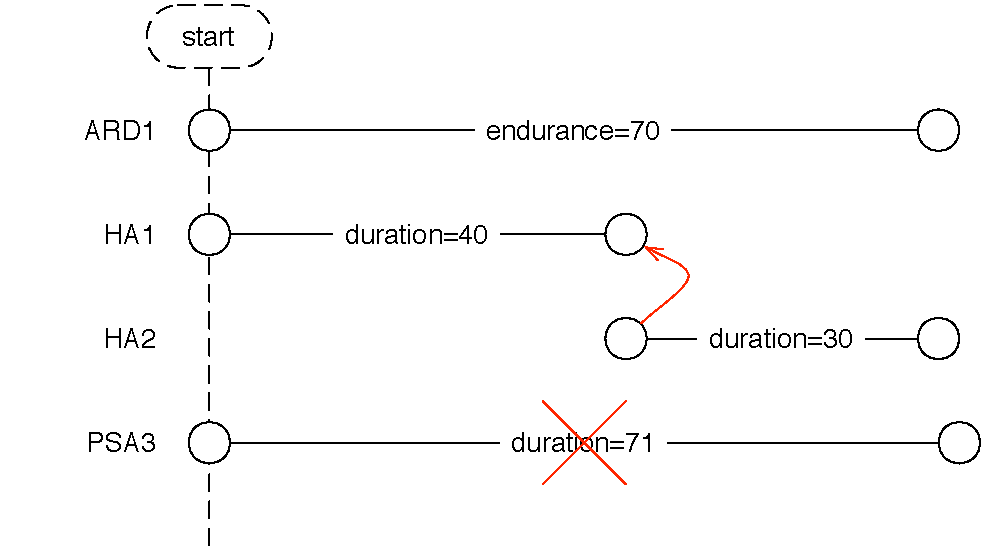
\includegraphics[scale=0.58]{img/mission-3g.pdf}
\caption[Mission 3g]{An illustration of Mission~3g, with red arrows representing preconditions and horizontal lines representing the passage of time. The \emph{x mark} denotes a point of failure for the mission.}
\label{fig:mission_3g}
\end{figure}

Finally, eight mission plans contained action workflow errors that resulted in deadlock. Figure~\ref{fig:mission_2d} illustrates this type of error with Mission~2d, which also belongs to the set of missions supporting our evaluation. Mission~2d comprises two assets with identifiers~\texttt{ARD1} and~\texttt{H1}, and three hover actions with identifiers \texttt{HA1}--\texttt{HA3}. The mission becomes deadlocked, and consequently fails, when the action workflow comprising~\texttt{HA1} and~\texttt{HA2} is disrupted. This disruption occurs because:

\begin{itemize}

\item \texttt{HA1} and~\texttt{HA2} are kinetic actions assigned to asset~\texttt{ARD1};

\item \texttt{HA1} and the cross-cutting action~\texttt{HA3}, which is assigned to asset~\texttt{H1}, are preconditions to~\texttt{HA2};

\item the duration of~\texttt{HA3} is greater than the duration of~\texttt{HA1}.

\end{itemize}

\begin{figure}[ht]
\centering
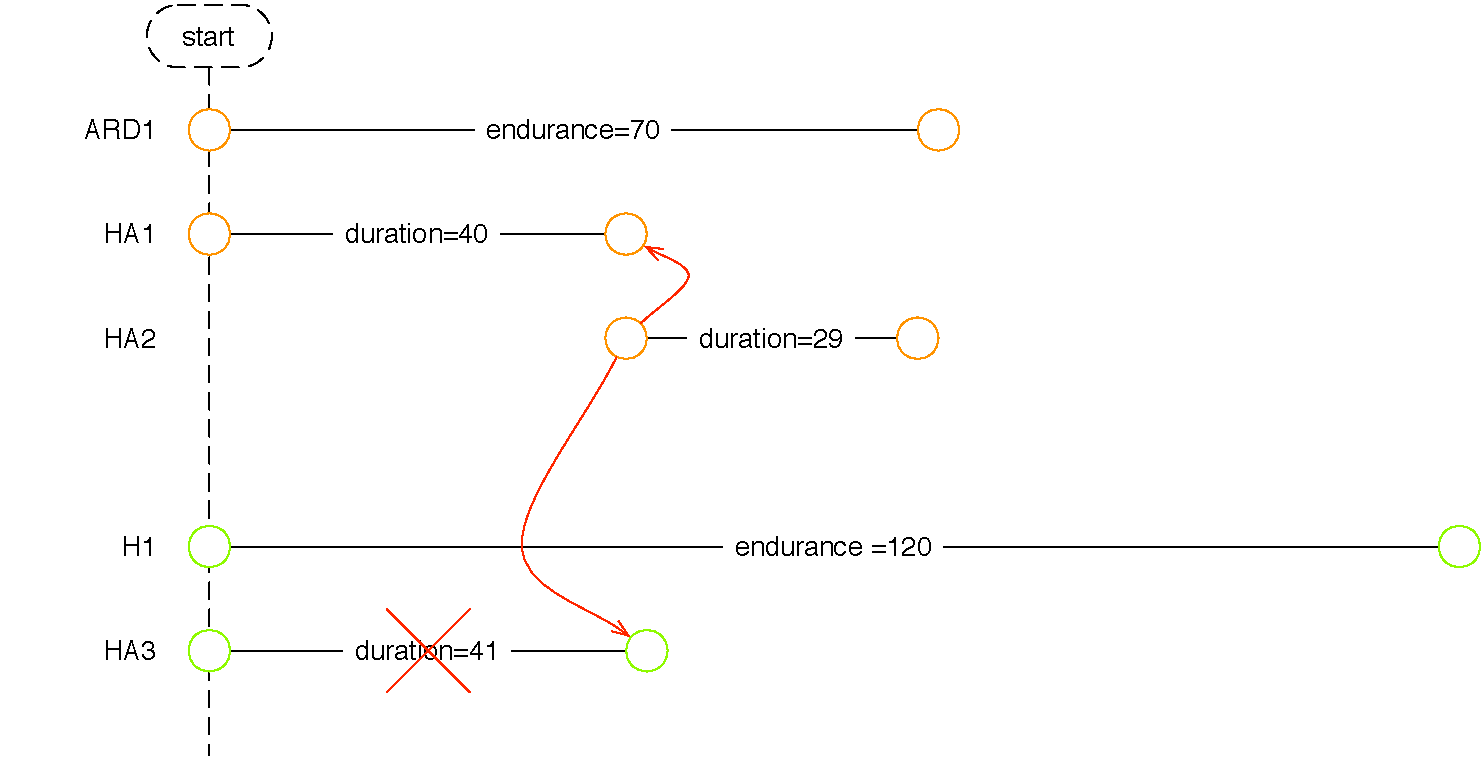
\includegraphics[scale=0.58]{img/mission-2d.pdf}
\caption[Mission 2d]{An illustration of Mission~2d, with red arrows representing preconditions and horizontal lines representing the passage of time. The \emph{x mark} denotes a point of failure for the mission. Color coded circles delineate the operation and execution of assets and actions, respectively, and group actions and the assets to which those actions are assigned.}
\label{fig:mission_2d}
\end{figure}

The propensity for cross-cutting actions to produce deadlock and thereby compromise mission correctness is associated with the degree of coupling between kinetic actions assigned to the same asset. The type of deadlock observed in Mission~2d is, to some extent, a consequence of tight coupling between the actions~\texttt{HA1} and~\texttt{HA2}, which are required by our behavioral model to execute continuously during the operation of \texttt{ARD1}. By eliminating the requirement for continuity, a looser coupling could permit~\texttt{HA2} to begin its execution after the end of~\texttt{HA3}. But missions comprising loosely coupled kinetic actions would still have to account for side effects resulting from potential workflow disruptions. For example, a loose coupling between~\texttt{HA1} and~\texttt{HA2} would enable the execution of~\texttt{HA3} to impose a hiatus on the workflow assigned to \texttt{ARD1}, with implications for the operation of that asset. We have chosen to avoid these implications, whose resolution would not have been straightforward, by establishing the deadlock in Mission~2d as a mission specification error.

The errors presented in this section were successfully identified by our prototype. While the correctness of some mission plans was absolute (with a~0.0 or~1.0 probability of success) several mission plans, including plans comprising threat area incursions, were associated with variable probabilities of success. For example, the probability of success for Mission~A is approximately~0.299 (as described in Section~\ref{sec:Synthesized_Models_and_Properties}).

\subsection{Proof of Correctness}

Given the broad range of disparate techniques described throughout this thesis, a formal proof of correctness for cascading verification may not be feasible. But correctness can be evaluated against simulations carried out during the behavioral modeling process. To this end, simulations were carried out during the development of the~58 mission plans. Simulated model executions are facilitated by the PRISM \emph{simulator}, a tool that generates sample paths through PRISM models. Partial simulation results for Mission~A are plotted by the graph in Figure~\ref{fig:mission_simulation}, where x-axis and y-axis represent variable values and time during specific executions, respectively; and plotted values represent endurance for asset~\texttt{H1} (variable~\texttt{e1}) and duration for the actions assigned to that asset (variables~\texttt{d1} and~\texttt{d2}).

\begin{figure}[ht]
\centering
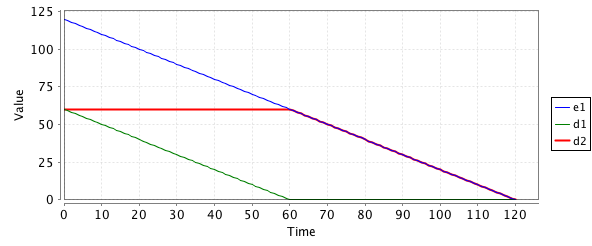
\includegraphics[width=\textwidth]{img/mission-simulation.png}
\caption[Mission simulation]{Partial simulation results for Mission~A\@. The x-axis and y-axis represent variable values and time during specific executions, respectively; and plotted values depict endurance for asset~\texttt{H1} (variable~\texttt{e1}) and duration for the actions assigned to that asset (variables~\texttt{d1} and~\texttt{d2}).}
\label{fig:mission_simulation}
\end{figure}

\section{Threats to Validity}
\label{sec:Threats_to_Validity}

This evaluation has thus far been concerned with the abstraction and effectiveness afforded by our method and prototype. Research can be evaluated further by considering threats to its validity. Threat types applicable to our research include conclusion validity, internal validity, construct validity and external validity~\cite{Wright_2010,Feldt_2010}.

Conclusion validity addresses the issue of correlation between the functionality afforded by our prototype and the correctness of UAV mission specifications, whereby correctness is determined with respect to specific properties of interest. We believe this correlation to be established by the results presented in Section~\ref{sec:Evaluation_Methods_and_Metrics}. To recap, in conjunction with the verification provided by PRISM, reduced LOC, tokens and potential (domain-specific and behavioral modeling) errors demonstrate that our method and prototype have a significant and positive effect on the correctness of UAV mission specifications.

\subsection{Internal Validity}

Having established correlation, we proceed to establish internal validity, which addresses the issue of causation between the functionality afforded by our prototype and the correctness of UAV mission specifications. For correlated variables~\emph{x} and~\emph{y}, it can be claimed that~\emph{x} causes~\emph{y} if~\emph{x} precedes~\emph{y} in the absence of \emph{confounding factors}~\cite{Seltman_2013}. We will not elaborate on the issue of precedence except to mention that our prototype's functionality precedes verification results returned by PRISM\@. The problem of confounding is somewhat more challenging.

Confounding can occur when unknown or extraneous factors affect the relationship between correlated variables. With well defined input and output interfaces, our prototype is not likely to be influenced by unknown factors. But the~58 mission plans that act as input to the prototype, and thereby generate the established correlation, could constitute an extraneous factor if they fail to 1) be grounded in the real-world, or 2) sample a sufficiently large subset of the UAV mission state space. The former concern is mitigated by the real-world mission scenarios underpinning our mission plans. The latter concern is related to the issue of variability.

We do not attempt to achieve variability with, for example, randomized mission parameters. Nevertheless, mission plans vary with respect to LOC and token values, as indicated in Table~\ref{tab:mission_metrics}. Mission plans also vary along several parameters, which are listed in Table~\ref{tab:mission_parameters} for a subset of the~58 mission plans. These parameters include numbers of assets; kinetic, sensor and cross-cutting actions; and preconditions and concurrencies. Concerns regarding the potential for mission plans to act as a confounding factor are therefore mitigated by the observed variability in both metric values and mission parameters.

\begin{table}[!ht]
	\arrayrulecolor{Gray}
	\renewcommand*\arraystretch{1.3}
	\begin{tabularx}{\textwidth}{
			>{\centering\hsize=0.08\hsize}X|
			>{\centering\hsize=0.11\hsize}X|
			>{\centering\hsize=0.11\hsize}X
			>{\centering\hsize=0.11\hsize}X
			>{\centering\hsize=0.19\hsize}X|
			>{\centering\hsize=0.2\hsize}X
			>{\centering\hsize=0.2\hsize}X
		}
		& & \multicolumn{3}{ c | }{\emph{actions}} &
				\multicolumn{2}{ c }{\emph{dependencies}}\tabularnewline
		id & assets & kinetic & sensor & cross-cutting & preconditions & concurrencies\tabularnewline
		\hline
		1a & 1 & 1 & 0 & 0 & 0 & 0 \tabularnewline
		1d & 1 & 2 & 0 & 0 & 1 & 0 \tabularnewline
		1g & 1 & 3 & 0 & 0 & 2 & 0 \tabularnewline
		2a & 2 & 3 & 0 & 0 & 1 & 0 \tabularnewline
		2b & 2 & 3 & 0 & 1 & 2 & 0 \tabularnewline
		2e & 3 & 4 & 0 & 2 & 3 & 0 \tabularnewline
		2g & 2 & 5 & 0 & 2 & 5 & 0 \tabularnewline
		2j & 2 & 5 & 0 & 1 & 4 & 0 \tabularnewline
		2m & 2 & 6 & 0 & 1 & 5 & 0 \tabularnewline
		2p & 2 & 6 & 0 & 2 & 6 & 0 \tabularnewline
		2r & 3 & 5 & 0 & 2 & 4 & 0 \tabularnewline
		2u & 3 & 6 & 0 & 2 & 5 & 0 \tabularnewline
		2v & 3 & 6 & 0 & 2 & 5 & 0 \tabularnewline
		2w & 3 & 7 & 0 & 2 & 6 & 0 \tabularnewline
		2x & 3 & 7 & 0 & 2 & 6 & 0 \tabularnewline
		3a & 1 & 1 & 1 & 0 & 0 & 0 \tabularnewline
		3e & 1 & 2 & 1 & 0 & 1 & 0 \tabularnewline
		3h & 1 & 2 & 1 & 0 & 2 & 0 \tabularnewline
		3k & 1 & 2 & 2 & 0 & 2 & 0 \tabularnewline
		3o & 1 & 2 & 2 & 0 & 3 & 0 \tabularnewline
		4a & 1 & 4 & 0 & 0 & 3 & 0 \tabularnewline
		4b & 1 & 4 & 0 & 0 & 3 & 0 \tabularnewline
		4d & 1 & 4 & 1 & 0 & 4 & 0 \tabularnewline
		4f & 1 & 4 & 2 & 0 & 5 & 0 \tabularnewline
		5a & 1 & 3 & 2 & 0 & 2 & 2 \tabularnewline
		5b & 1 & 3 & 2 & 0 & 2 & 2 \tabularnewline
	\end{tabularx}
	\caption[Mission plan parameters]{Parameters---including number of assets, actions and action dependencies---for the representative mission plans listed in Table~\ref{tab:mission_metrics}.}
	\label{tab:mission_parameters}
\end{table}

The size of DTMC and PCTL templates could constitute a second extraneous factor if PRISM-to-YAML ratios are affected by poor template design rather than the functionality afforded by our prototype. But this is not the case: our templates are not designed to create code bloat, but rather to generate PRISM code that is intelligible to a human model builder. We also note that metric values in Table~\ref{tab:mission_metrics} do not account for programmer-readable comments.

\subsection{Construct Validity}

Construct validity addresses the metrics, including LOC and token count, used to quantify model and property specification complexity. These are widely applicable, language independent software metrics that ignore logic structure and control flow. The ability to bypass control flow is useful when evaluating complexity in the context of the PRISM language, a somewhat unconventional formalism that lacks appropriate control structures.

We do acknowledge that a LOC- and token-based analysis cannot in and of itself account for the intricate syntax of the PRISM language. To address this limitation, we propose a multidimensional complexity model~\cite{Kaner_2004}, which encompasses domain-specific and behavioral modeling errors prevented by our prototype. The (potentially bidirectional) correlation between error rates and software complexity suggests that software errors can be used as descriptors of complexity~\cite{Banker_1989,Kan_2002}. By considering complexity from multiple dimensions, our metric- and error-based analysis provides a more complete understanding of PRISM artifact complexity, which in turn increases confidence in the resulting evaluation.

\subsection{External Validity}

Finally, we consider external validity, which addresses the issue of transferability/portability. In conjunction with the complexity of the UAV domain, and the real-world DARPA and DRDC mission scenarios underpinning this evaluation, the results presented in Section~\ref{sec:Evaluation_Methods_and_Metrics} suggest that cascading verification can be ported to different application domains. The portability of our method is supported by the general purpose of its constituent technologies including OWL+SWRL, Prolog, and DTMC and PCTL\@. Presently, we cannot make the same argument for the \emph{connections} that link those technologies in the context of the method. But cascading verification is an extension of semantic model checking methods with identical or comparable constituent technologies (similarities to semantic model checking were presented in Section~\ref{sec:Cascading_Verification_Related_Work}). The successful application of these methods to the Web service domain further supports the portability of cascading verification.

\section{Summary}
\label{sec:Evaluation_Summary}

By automating the synthesis of PRISM artifacts, and by providing multiple stages of reasoning and analysis, our prototype enhances the abstraction level of model and property specifications, and the effectiveness of probabilistic model checking, respectively. This cascading approach to verification improves mission correctness to a degree that is evidently unattainable by the individual components that constitute the prototype.

We note that this evaluation is preliminary. Further work is required to determine the utility of our prototype in the context of a more sophisticated mission specification language and domain model; and the ability of cascading verification to support probabilistic model checking in the context of other non-trivial domains.
